\chapter{Abschätzung systematischer Unsicherheiten} \label{kap:systematik}
Der Fitter liefert zwar eine statistische Unsicherheit auf $\SJPsi$, allerdings ist eine Betrachtung der Systematik unerlässlich. Im Folgenden wird daher der Einfluss einiger Effekte auf das Fitergebnis untersucht und anschließend der systematische Fehler abgeschätzt.

\section{Fitmethode} \label{kap:fit_bias}
Die hier verwendete Maximum-Likelihood-Methode hat zwar den schönen Vorteil, dass das Fitergebnis nicht von der Einteilung des Histogramms abhängt, es ist jedoch nicht von vornherein ausgeschlossen, dass sie das Ergebnis verfälscht (einen sog. Bias produziert). Daher wird eine Toy Monte Carlo - Studie (kurz: Toy MC) durchgeführt. Dabei werden Daten zufällig nach einer Verteilung mit den gewünschten Parametern generiert und im Anschluss gefittet. Zur Generation der Massen- und Eigenzeitverteilung werden die aus den Fits erhaltenen Parameter verwendet (siehe Tabellen \ref{tab:fit_masse} und \ref{tab:fit_results}). Die einzige Ausnahme bildet $\SJPsi$, da diese zum Zeitpunkt dieser Studie noch verdeckt war. Hier wurde mit $\SJPsi = 0,75$ generiert. Entsprechend der Statistik im verwendeten Datensatz werden hier jeweils 13000 Ereignisse generiert. Durch mehrmaliges Wiederholen von Generation und Fit sollten die gefitteten Parameter am Ende gaußverteilt um die in der Generation verwendeten Parameter sein. Kommt es zu Abweichungen davon, so ist dies auf die Fitmethode oder eine fehlerhafte Implementation des Eperimentators zurückzuführen. Um statistisch zuverlässige Aussagen treffen zu können, wurden in dieser Toy MC - Studie insgesamt 20000 Wiederholungen durchgeführt.

\begin{figure}[hptb]
\centering
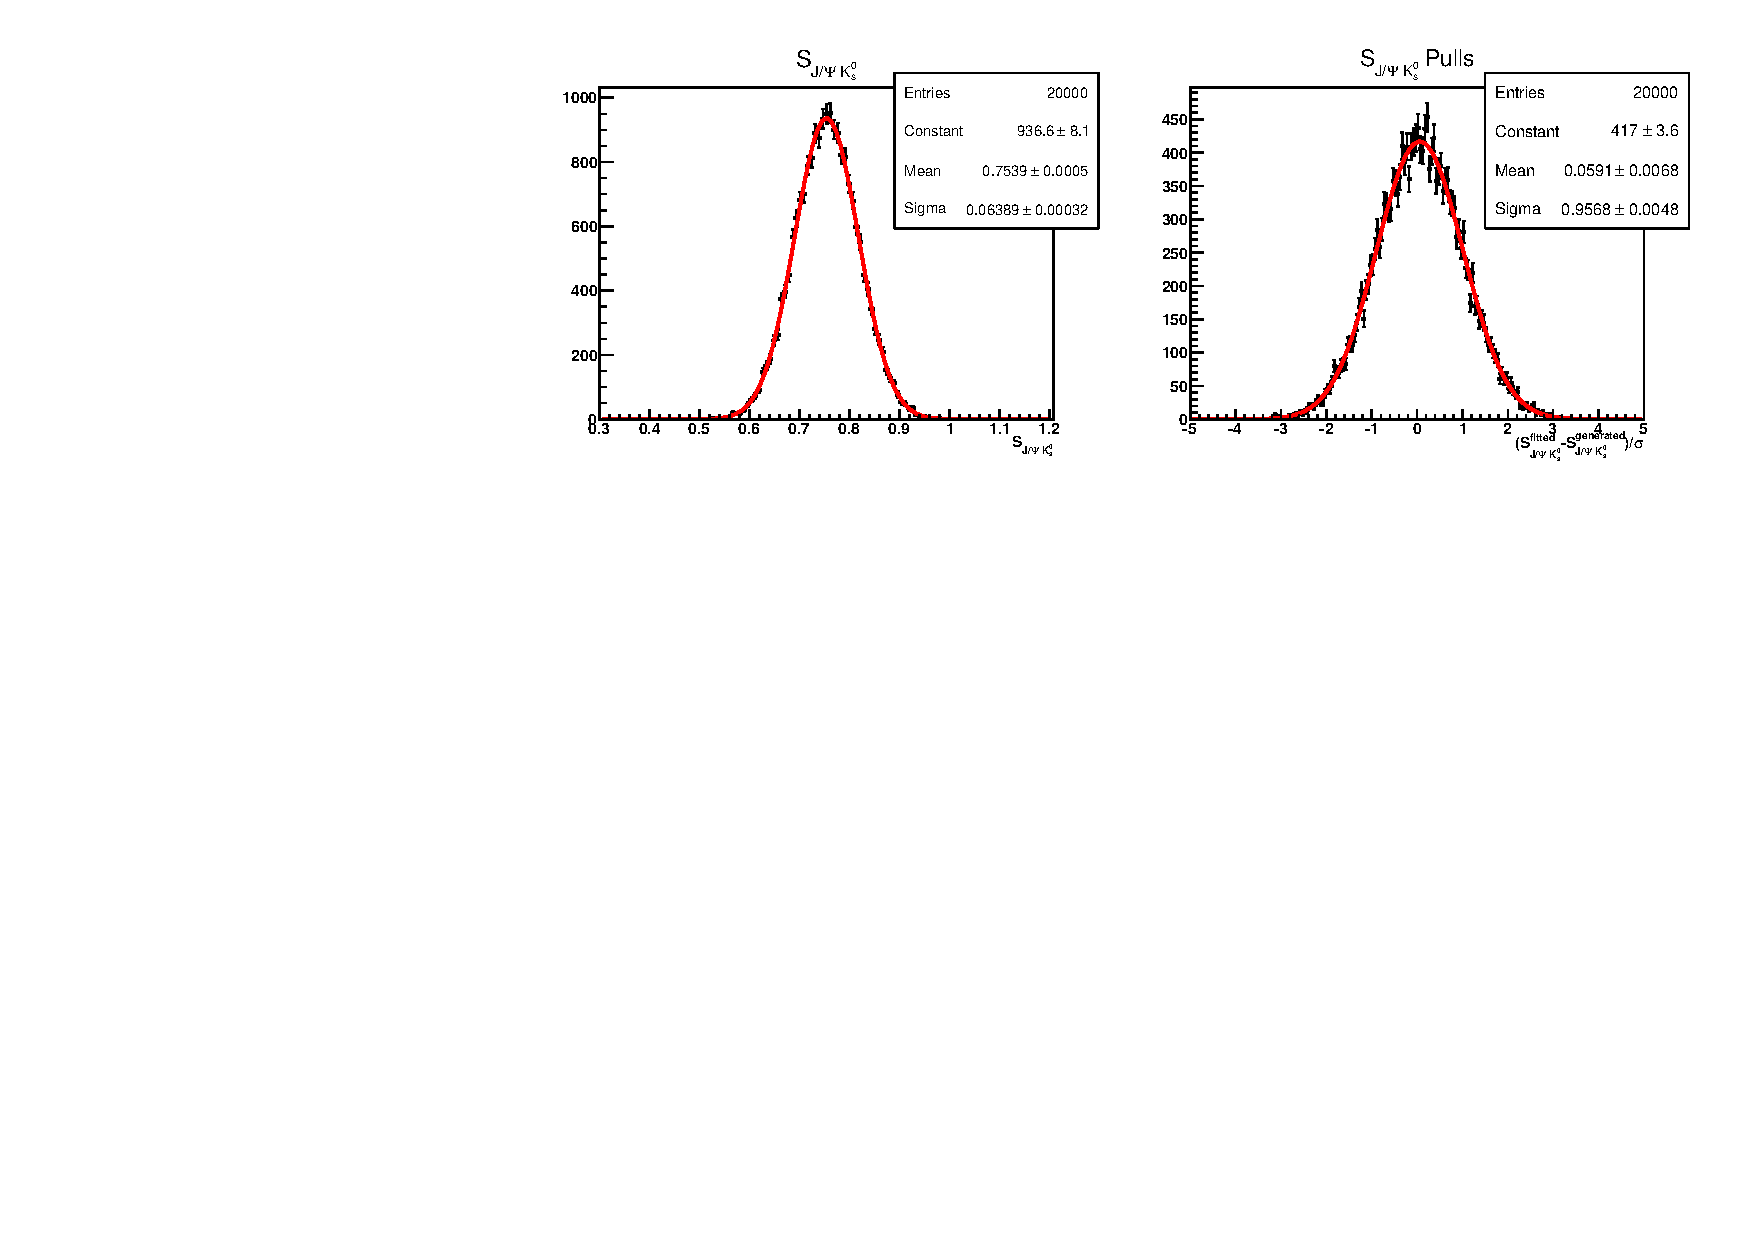
\includegraphics[width = 0.6\textwidth]{fit_bias}
\caption{Verteilung der aus der Toy MC Studie erhaltenen Amplituden $\SJPsi$ (links) sowie die dazugehörigen Pulls (rechts)}
\label{fig:fit_bias}
\end{figure}

Abbildung \ref{fig:fit_bias} zeigt sowohl die Verteilung der gefitteten Amplitude $\SJPsi$ als auch die Pulls, die sich mittels $\frac{\SJPsi^{gefittet} - \SJPsi^{generiert}}{\sigma^{gefittet}}$ berechnen lassen. Der Mittelwert der Amplitudenverteilung (links) $\SJPsi^{\text{ToyMC}} = 0,7548 \pm 0,0005$ weicht signifikant vom generierten Wert $\SJPsi = 0,75$ ab, es gibt also einen Bias. An der Pull-Verteilung lassen sich prinzipiell zwei Dinge beobachten:
\begin{enumerate}
    \item An der Verschiebung des Pull-Mittelwertes $\mu = 0,0679 \pm 0,0067$ von der Null sieht man deutlich, dass es - wie bereits erwähnt - einen kleinen, aber signifikanten Bias gibt. Indem dieser Bias mit der statistischen Unsicherheit aus dem Fitergebnis (siehe Gl. \ref{eq:fit_result}) multipliziert wird, erhält man eine Abschätzung der aus der Fitmethode resultierenden Unsicherheit:
        \begin{align}
        \delta\SJPsi^{Fit} = 0,0679 \cdot 0,069 = 0,0047
        \end{align}

    \item Mit einem $\sigma = 0,9462 \pm 0,0047$ ist die Pull-Verteilung signifikant zu schmal. Dies bedeutet, dass der Fit den statistischen Fehler überschätzt. Weitere Untersuchungen zeigen, dass Problem auftritt, sobald man in den Toys Untergrund miteinbezieht (siehe Abb. \ref{fig:toys_no_bkg}). Es ist bekannt, dass die verwendete sFit-Methode die Fehlerpropagation (gerade bei Untergrund) nicht korrekt ausführt. Es wurde vom Betreuer eine Fehlerkorrektur implementiert, dabei handelt es sich jedoch um eine Näherung. Für eine tiefergehende Studie müsste die Fehlerkorrektur entsprechend analysiert werden.
\end{enumerate}

\subsubsection{Ursachen des Bias}
!!! nochmal bearbeiten !!!

Es bleibt zu klären, welche Ursachen zu dem Bias führen. Dazu wird zunächst eine Toy MC-Studie ohne Untergrund ($f_{sig}=1$) durchgeführt
Weitere Toy MC Studien zeigen, dass die Behandlung des Untergrundes zu einem Bias führt. Generiert man nämlich nur Signal, ist der Mittelwert kompatibel zur Null (siehe Abb. \ref{fig:toys_no_bkg}).

\begin{figure}[hptb]
\centering
%\includegraphics[width=\textwidth]{}
\caption{Toy MC Studie mit reinem Signal ohne Untergrund. Es kommt zu keinem signifikanten Bias. Links: Verteilung der erhaltenen Amplitude, Rechts: Pull-Verteilung.}
\label{fig:toys_no_bkg}
\end{figure}

Die Vermutung ist, dass zu wenig Statistik im Fit die eigentliche Ursache für den Bias ist. Daher wurden weitere Toy MC Studien mit unterschiedlicher Anzahl an Teilchen pro Toy durchgeführt. Die Ergebnisse sind in Tabelle \ref{tab:fit_bias_events} aufgeführt und in Abbildung \ref{fig:fit_bias_events} nochmals visualisiert. Man sieht, dass sich der Fit Bias mit erhöhter Statistik deutlich reduzieren lässt. Allerdings lässt das Ergebnis Zweifel aufkommen, ob er sich mit noch mehr Statistik gänzlich verschwindet.

\begin{table}[hptb]
\centering
\caption{Toy MC Studien mit unterschiedlicher Anzahl an generierten Events pro Toy. Genannt wird der Mittelwert $\mu$ der $\SJPsi$-Pull-Verteilung}
\label{tab:fit_bias_events}
\begin{tabular}{cr@{$\pm$}l}
\hline \hline 
Teilchen pro Toy & \multicolumn{2}{c}{$\mu$}  \\ \hline
20000            &  0,059 & 0,007 \\
50000            &  0,036 & 0,007 \\
100000           &  0,020 & 0,007 \\
200000           &  0,022 & 0,007 \\ 
\hline \hline
\end{tabular}
\end{table}

\begin{figure}[hptb]
\centering
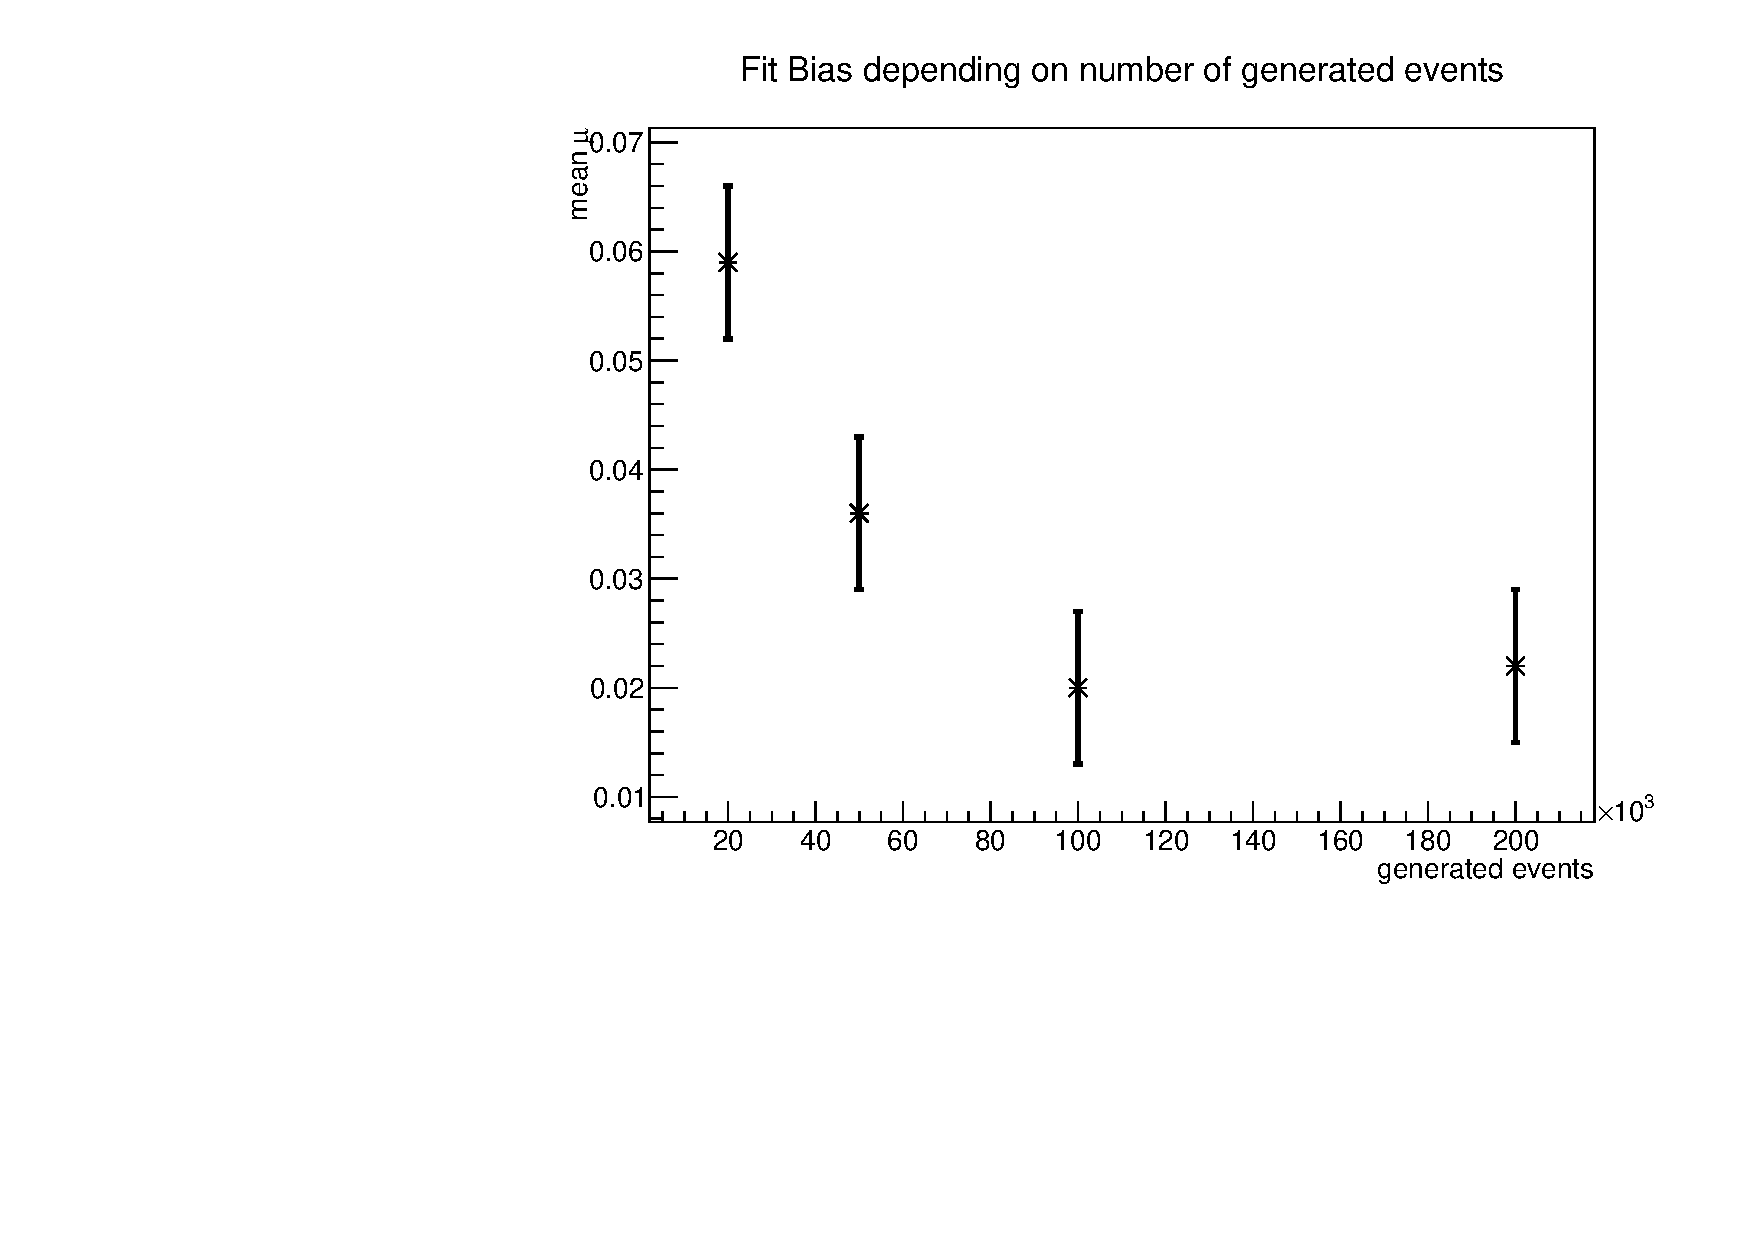
\includegraphics[width=\textwidth]{fit_bias_statistics}
\caption{Toy MC Studien mit unterschiedlicher Anzahl an generierten Events pro Toy. Als Maß für den Fit Bias dient der Mittelwert $\mu$ der $\SJPsi$-Pull-Verteilung}
\label{fig:fit_bias_events}
\end{figure}

\section{Kalibration des Taggings}
Im Fit wird bei den Parametern der Tagging Kalibration nur der statistischen Fehler berücksichtigt. Es soll nun an dieser Stelle der Einfluss der statistischen Unsicherheiten abgeschätzt werden. \\
Die Korrekturparameter $p_0$ und $p_1$ für die Fehlerwahrscheinlichkeit des OST sind gegeben durch
\begin{align}
p_0 &= 0,392 \pm 0,0017\ \text{(stat.)} \pm 0,0076\ \text{(syst.)} \\
p_1 &= 1,035 \pm 0,021\ \text{(stat.)} \pm 0,0076\ \text{(syst.)}.
\end{align}

\paragraph{Variation der Parameter in den Daten}
!!! Wichtig !!! - Dieser Abschnitt muss nochmal überarbeitet werden. (Werte anpassen)

Zunächst werden die Startwerte der Parameter $p_0$ und $p_1$ variiert, indem man jeweils den systematischen Fehler der Parameter addiert bzw. subtrahiert und dann den Fit auf die Daten durchührt. Für alle vier Kombinationen wird dann die Abweichung vom regulären Fitergebnis für $\SJPsi$ berechnet. Der Referenzwert aus dem Fit beträgt
\begin{align}
\SJPsi = 0,625 \pm 0,069
\end{align}

\begin{table}[hptb]
\centering
\caption{Variation des Fitergebnisses für $\SJPsi$ bei Veränderung der Startwerte für $p_0$ und $p_1$ $\pm$ ihrer statistischen Unsicherheiten}
\label{tab:syst_fit_calib_data}
\begin{tabular}{cc|r@{$\pm$}l|r@{$\pm$}l}
\hline\hline
$p_0$  &  $p_1$  &  \multicolumn{2}{c}{$\SJPsi$}  & \multicolumn{2}{c}{$\Delta\SJPsi$}   \\ \hline
0,3783 - 0,0028  &  0,950 - 0,028  &  0,7623 & 0,0005  &   0,0093 & 0,0007 \\
0,3783 + 0,0028  &  0,950 - 0,028  &  0,7368 & 0,0005  &  -0,0171 & 0,0007 \\
0,3783 - 0,0028  &  0,950 + 0,028  &  0,7729 & 0,0005  &   0,0190 & 0,0007 \\
0,3783 + 0,0028  &  0,950 + 0,028  &  0,747  & 0,001   &  -0,007  & 0,001 \\
\hline\hline
\end{tabular}
\end{table}

Die Ergebnisse sind Tabelle \ref{tab:syst_fit_calib_data} zu entnehmen. Die größte Abweichung beträgt hier $\Delta\SJPsi = 0,0190$.

\paragraph{Variation der Parameter in Toy MC}
Eine weitere Möglichkeit der Abschätzung besteht darin, sich entsprechende Toys zu generieren und diese dann zu fitten. Im Folgenden werden bei der Toy Generierung die Parameter $p_0$ und $p_1$ um ihre statistischen Unsicherheiten variiert (systematische Fehler auf die Kalibration liegen leider noch nicht vor), der Fit dann allerdings mit den ursprünglichen Parameterwerten durchgeführt. Als Referenzwert dient die aus dem Fit Bias (siehe Kapitel \ref{kap:fit_bias}) erhaltene Amplitude, da hier mit den regulären Parametern $p_0$ und $p_1$ generiert und gefittet wurde:

\begin{align}
\SJPsi = 0,7539 \pm 0,0005
\end{align}

\begin{table}[hptb]
\centering
\caption{Variation des Fitergebnisses für $\SJPsi$ bei Veränderung der Parameterwerte $p_0$ und $p_1$ $\pm$ ihrer statistischen Unsicherheiten bei der Generierung von Toys}
\label{tab:syst_fit_calib_toys}
\begin{tabular}{cc|r@{$\pm$}l|r@{$\pm$}l}
\hline\hline
$p_0$  &  $p_1$  &  \multicolumn{2}{c}{$\SJPsi$}  & \multicolumn{2}{c}{$\Delta\SJPsi$}   \\ \hline
0,3783 - 0,0028  &  0,950 - 0,028  &  0,7623 & 0,0005  &   0,0093 & 0,0007 \\
0,3783 + 0,0028  &  0,950 - 0,028  &  0,7368 & 0,0005  &  -0,0171 & 0,0007 \\
0,3783 - 0,0028  &  0,950 + 0,028  &  0,7729 & 0,0005  &   0,0190 & 0,0007 \\
0,3783 + 0,0028  &  0,950 + 0,028  &  0,747  & 0,001   &  -0,007  & 0,001 \\
\hline\hline
\end{tabular}
\end{table}

Die Ergebnisse sind Tabelle \ref{tab:syst_fit_calib_toys} zu entnehmen, diese wurde aus den Plots in Abbildung \ref{fig:toys_tag_calib}. Die größte Abweichung beträgt hier $\Delta\SJPsi = 0,0190$. Daher wird der systematische Fehler durch die Tagging Kalibrierung wie folgt abgeschätzt:

\begin{align}
\delta\SJPsi^{Tagging Kalibration} = 0,0190 \ .
\end{align}

\begin{figure}[hptb]
\subfigure[{$p_0 - \Delta p_0$,  $p_1 - \Delta p_1$}]{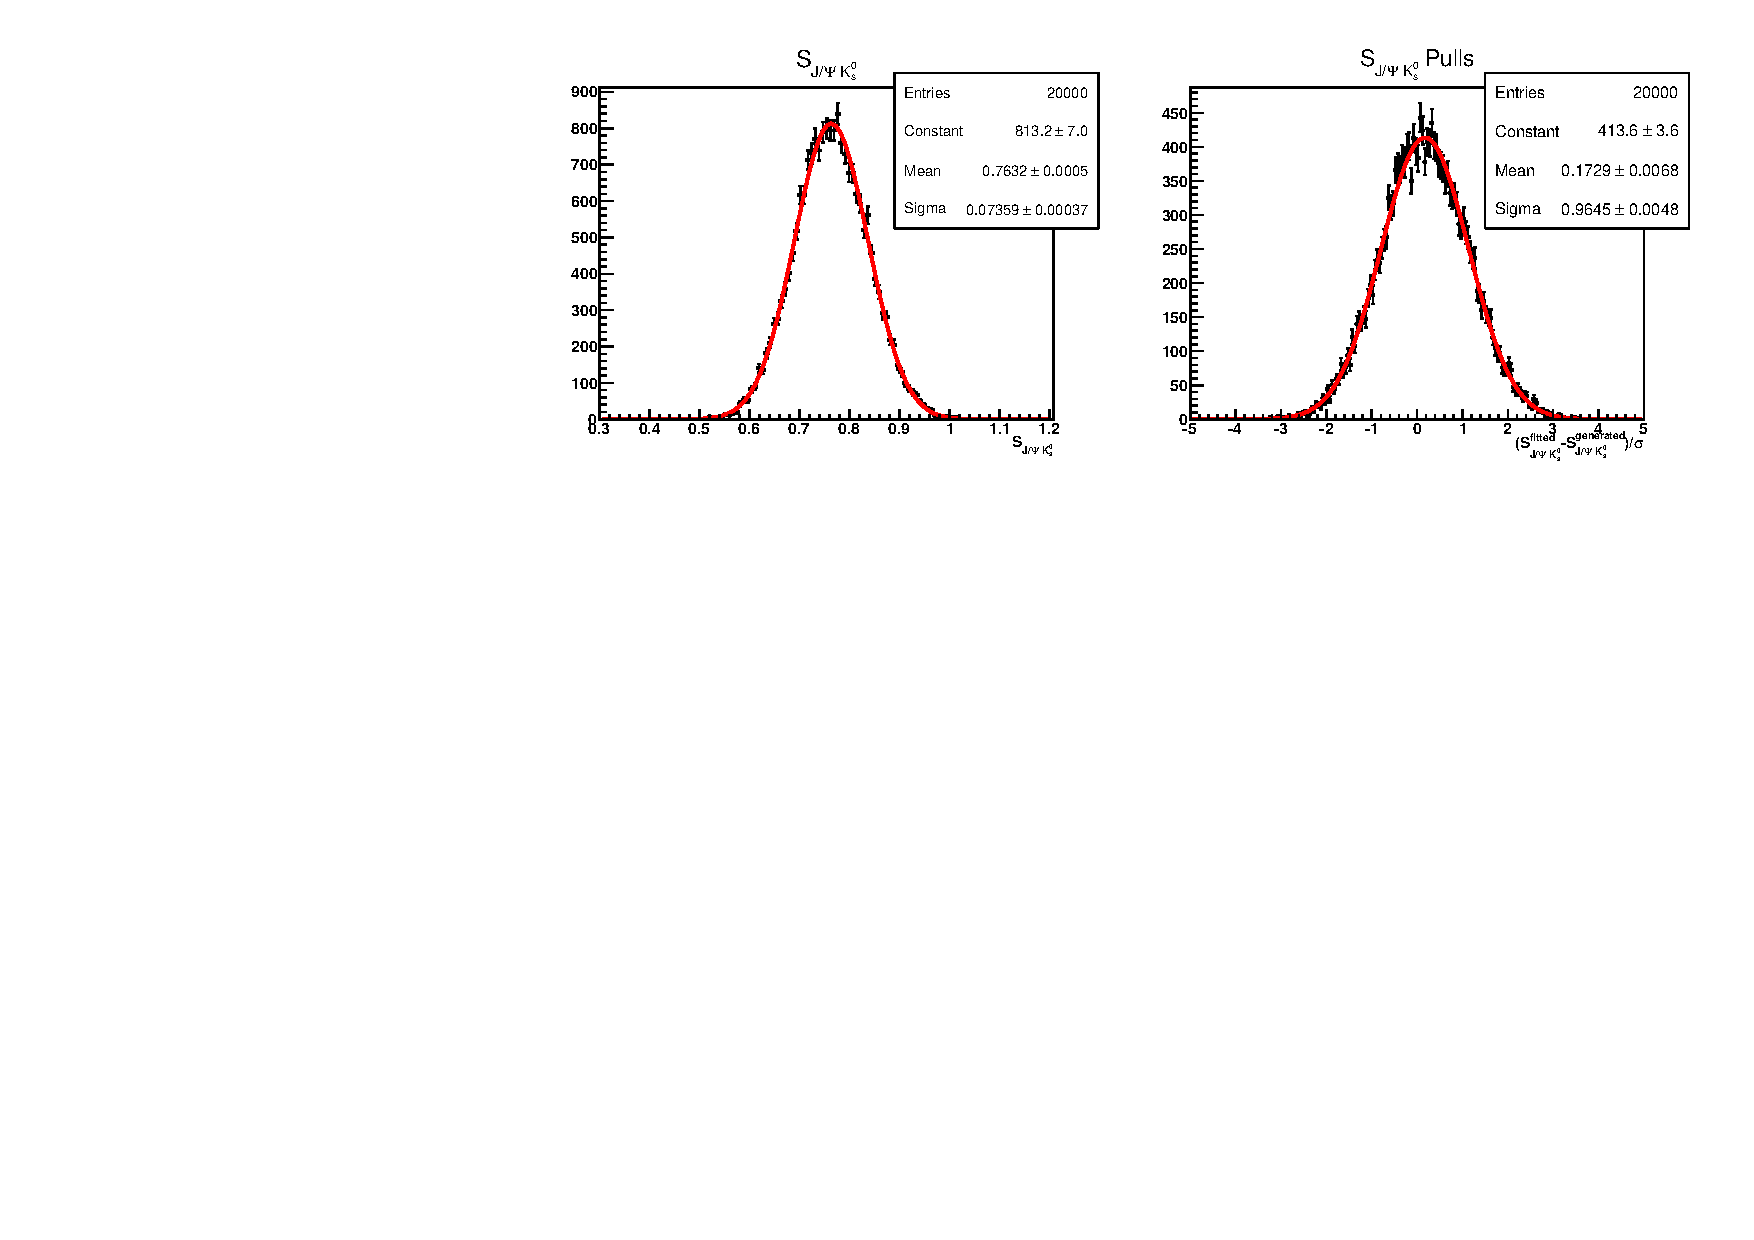
\includegraphics[width=0.7\textwidth]{tagging_calibration--}}
\subfigure[{$p_0 + \Delta p_0$,  $p_1 - \Delta p_1$}]{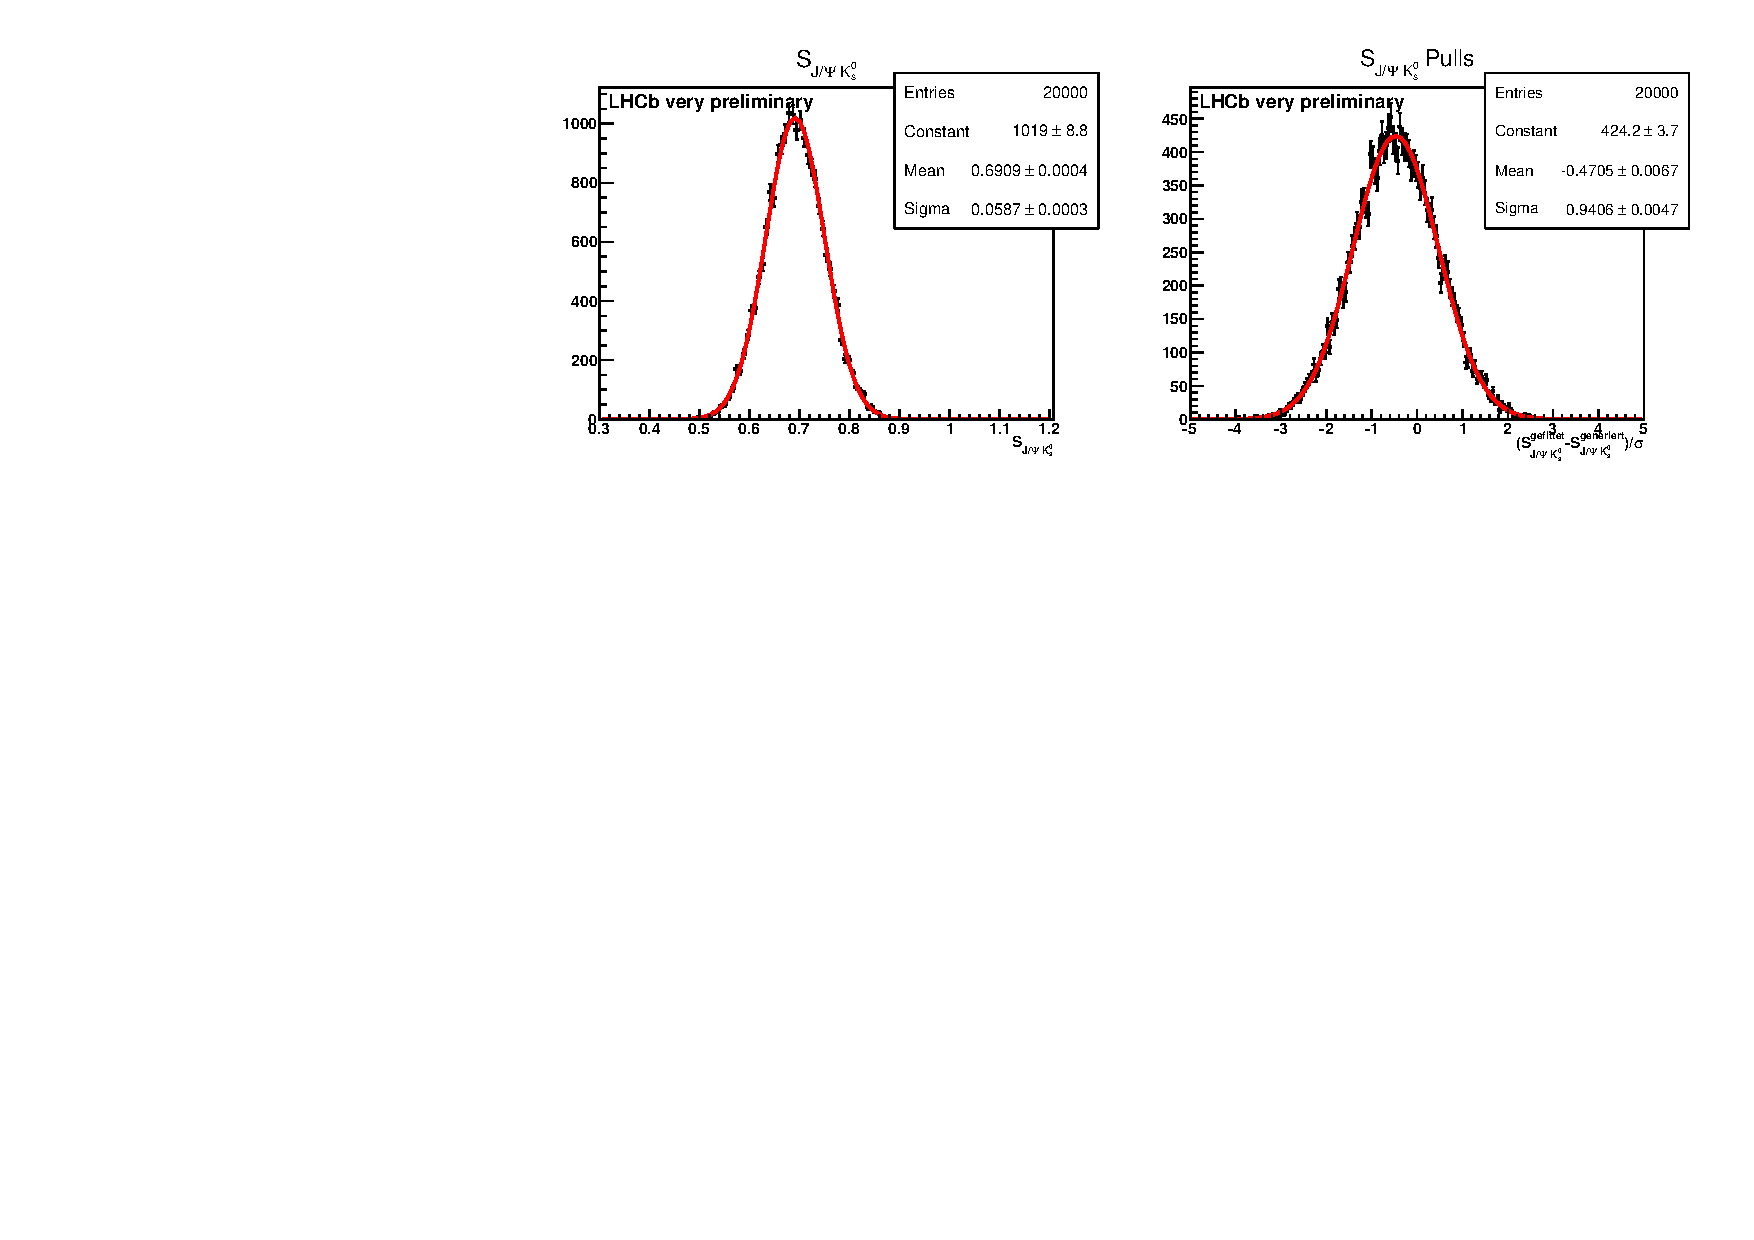
\includegraphics[width=0.7\textwidth]{tagging_calibration+-}}
\subfigure[{$p_0 - \Delta p_0$,  $p_1 + \Delta p_1$}]{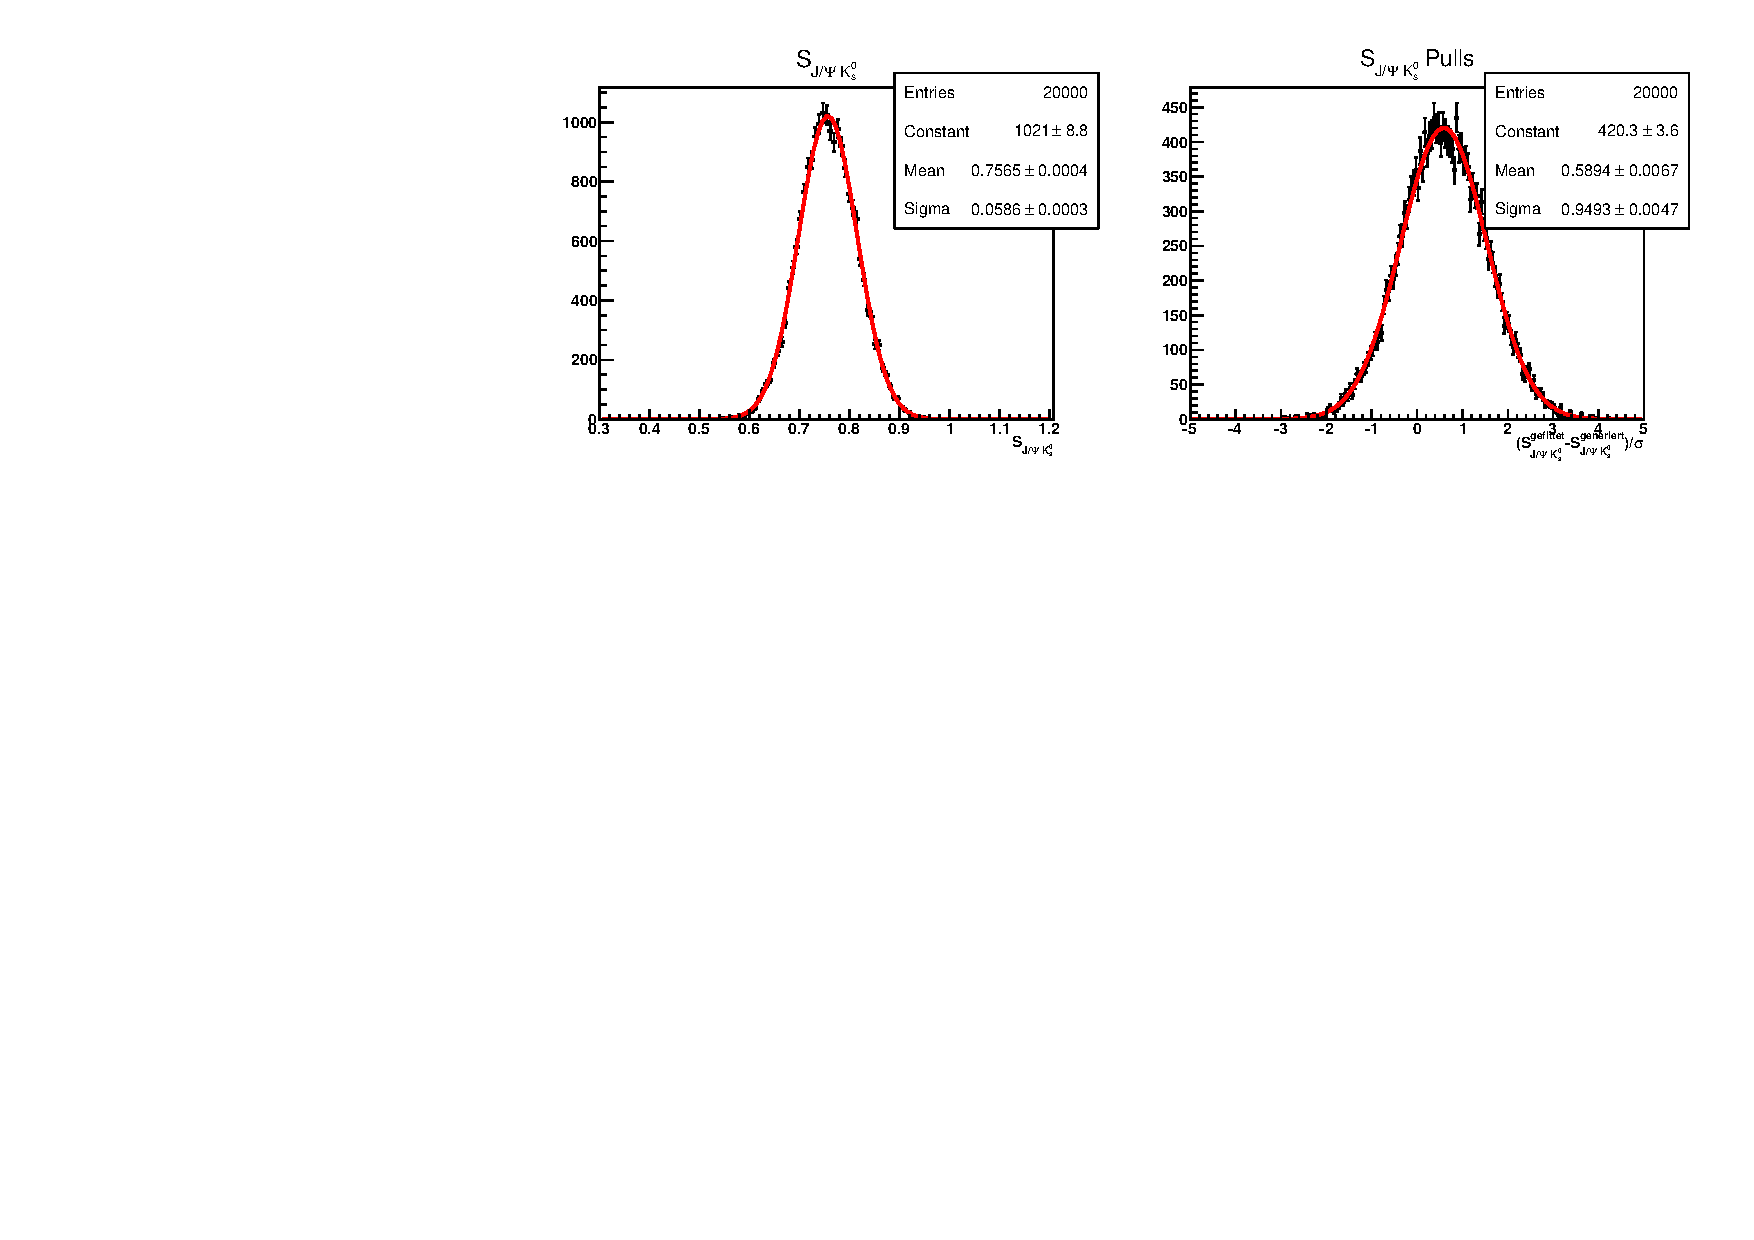
\includegraphics[width=0.7\textwidth]{tagging_calibration-+}}
\subfigure[{$p_0 + \Delta p_0$,  $p_1 + \Delta p_1$}]{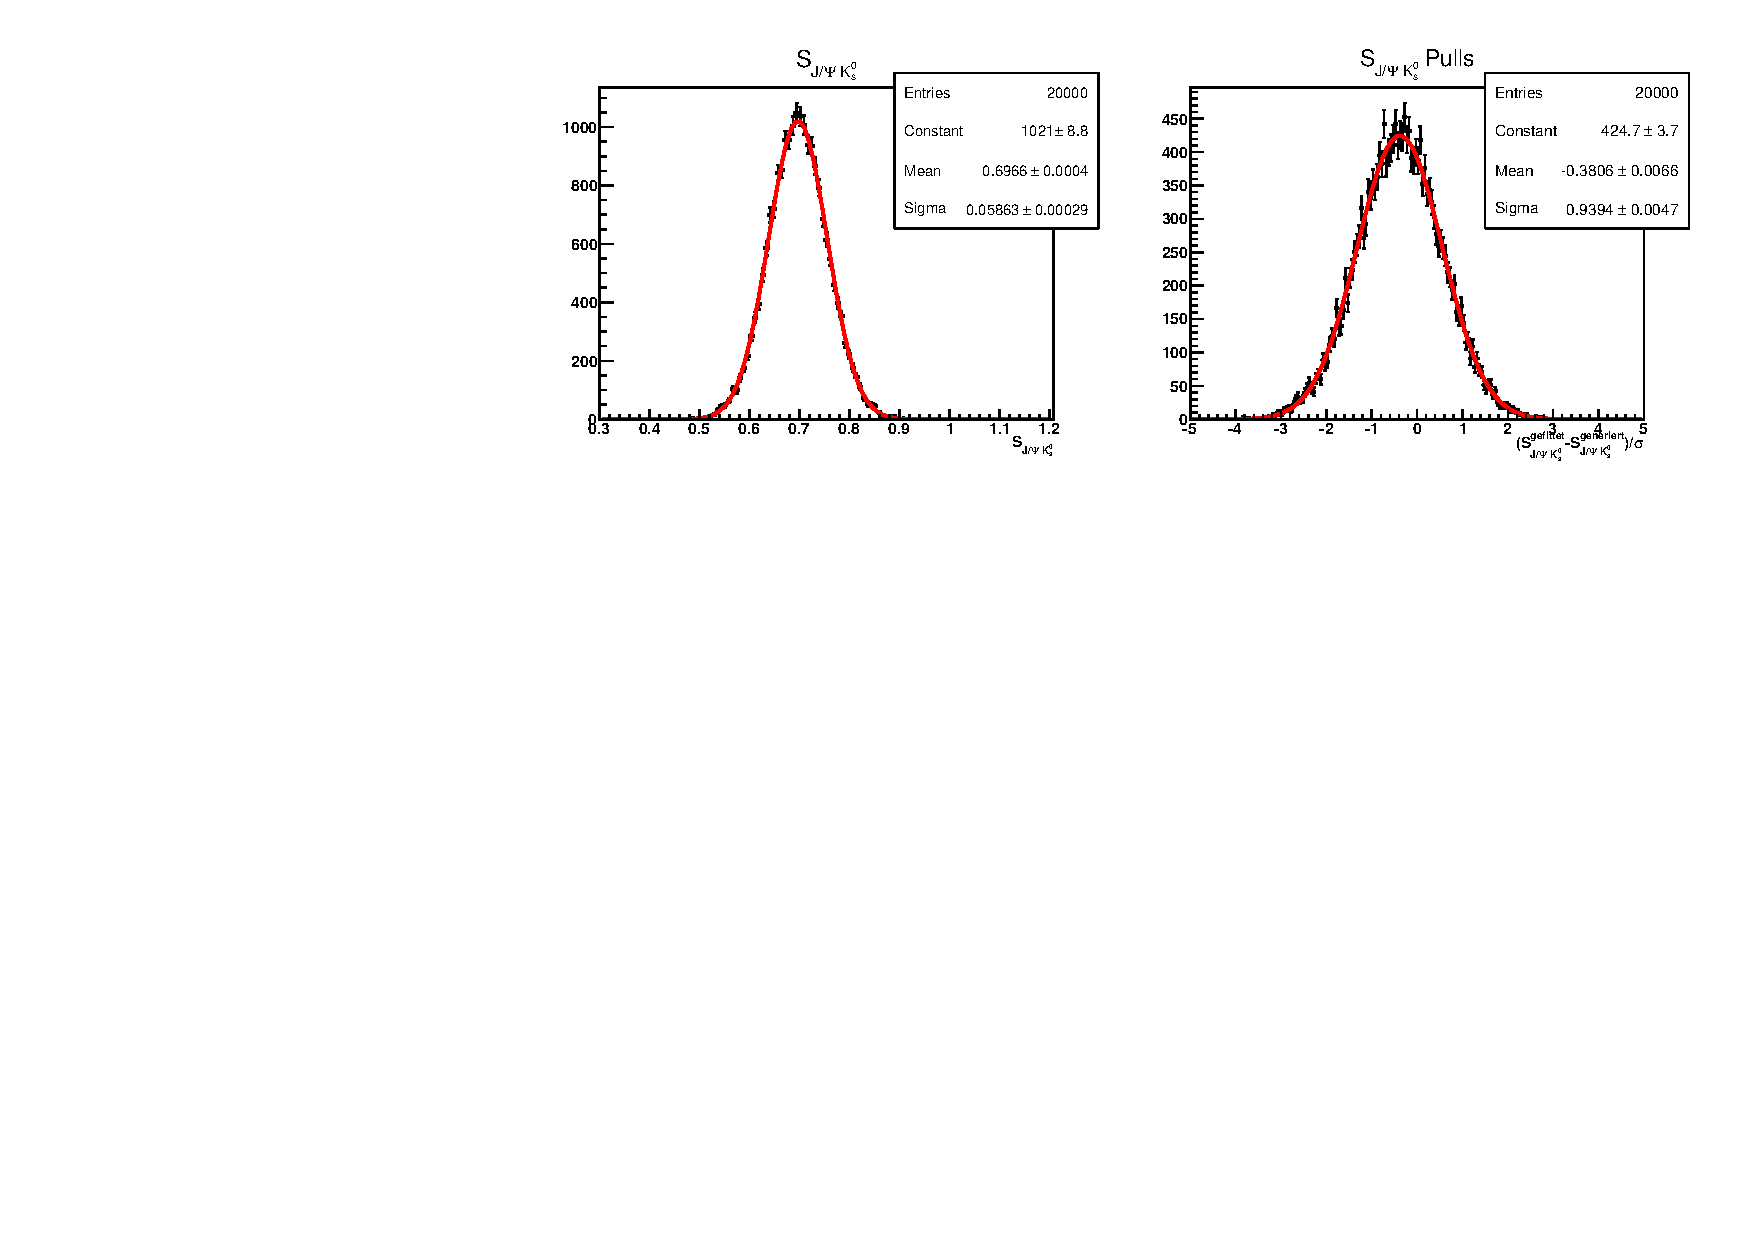
\includegraphics[width=0.7\textwidth]{tagging_calibration++}}
\caption{Toy MC Studie zur Abschätzung der Systematik durch die Tagging Kalibration. Bei der Generation wurden die Taggingparameter $p_0=0,3783$ und $p_1=0,950$ um ihre statischen Unsicherheiten $\Delta p_0 = 0,0028$ bzw. $\Delta p_1 = 0,028$ variiert, der Fit wurde dann mit den ursprünglichen Werten $p_0$ und $p_1$ durchgeführt.}
\label{fig:toys_tag_calib}
\end{figure}



\section{Einfluss einer zeitabhängigen Akzeptanz} \label{kap:akzeptanz}
In der Analyse wurde der Einfluss einer zeitabhängigen Detektorakzeptanz vernachlässigt. Nimmt man an, dass sich die Akzeptanz von \Bd- und \Bdbar-Mesonen nicht unterscheiden, so hat die Akzeptanz keinen Einfluss auf die Asymmetrie, da sie sich hier herauskürzt. Beim Fit der Amplitude nach Gleichung \ref{eq:fit_pdf} ist dies aber nicht zwangsläufig so. Um hiesiges Vorgehen zu rechtfertigen, wird zunächst eine Bestimmung der Akzeptanz durchgeführt und anschließend mit einer Toy MC Studie ihr Einfluss überprüft.

\subsection{Bestimmung der Akzeptanzfunktion} \label{kap:akzeptanz_bestimmung}
\Bd-Mesonen haben eine relativ lange Lebensdauer. Um sie von kurzlebigem Untergrund zu unterscheiden, befinden sich auf den Triggern und dem Stripping entsprechende Cuts auf die Flugzeiten. Dies hat zur Folge, dass für kleine Flugzeiten ($ct \lesssim 0,3\pico\second$) kaum \Bd-Mesonen im Detektor registriert werden und es zu einem sog. \glqq Turn-On-Effekt\grqq kommt. Es hat sich herausgestellt (\cite{lhcb-paper}), dass dieser gut durch die Funktion
\begin{align}
\epsilon_1(t) = \frac{2}{\pi}\arctan[t\cdot \exp(at+b)]
\end{align}
parametrisiert wird.

Je länger ein \Bd-Meson lebt, desto schwieriger wird es, die Zerfallsprodukte im Detektor auf Grund seiner begrenzten Länge nachzuweisen. Daher nimmt die Akzeptanz zu großen Zeiten hin wieder ab. Zur Parametrisierung fällt die Wahl auf eine lineare Funktion
\begin{align}
\epsilon_2(t) = 1 + \beta t \qquad (\beta < 0).
\end{align}

Die entsprechende gesamte Akzeptanzfunktion lautet demnach:
\begin{align}
\epsilon(t) = \epsilon_1(t) \cdot \epsilon_2(t) = \frac{2}{\pi}\arctan[t\cdot \exp(at+b)](1 + \beta t)
\end{align}

Zur Bestimmung der Paramater wird die Trennung von \Bd- und \Bdbar-Mesonen aufgehoben, sodass lediglich ein exponentieller Zerfall zu beobachten ist. Des weiteren wird der Cut auf die Lebensdauer bei $0,3\pico\second$ nicht angewandt, sodass der Turn-On-Effekt auch richtig sichtbar wird. Die Wahrscheinlichkeitsdichtefunktion für den Fit lautet somit:
\begin{align}
\mathcal{P}_{acc}(t) \propto \epsilon(t)\cdot \e^{-t/\tau} = \e^{-t/\tau}\cdot\frac{2}{\pi}\arctan[t\cdot \exp(at+b)](1 + \beta t)
\end{align}

Die beiden Parameter $\tau$ und $\beta$ sind stark miteinander korreliert. Für eine geeignete Bestimmung der Parameter der Akzeptanz-Funktion wird daher die Lebensdauer auf den PDG-Wert $\tau = 1,519 \pm 0,007 \pico\second$ \cite{pdg-tau} constraint, die anderen Parameter fließen. Die Ergebnisse sind in Tabelle \ref{tab:fit_akzeptanz} aufgeführt, die entsprechenden Plots in Abbildung \ref{fig:fit_akzeptanz}. 

\begin{table}[hptb]
\centering
\caption{Ergebnis des Fits zur Bestimmung der zeitlichen Akzeptanz}
\label{tab:fit_akzeptanz}
\begin{tabular}{lr@{$\pm$}l}
\hline \hline 
Parameter & \multicolumn{2}{c}{Ergebnis}  \\ \hline
$\tau$    &  1,519   & 0,007 \\
$a$       &  44,1    & 5,7 \\
$b$       &  -7,4    & 1,1 \\
$\beta$   &  -0,0056 & 0,0085 \\ 
\hline \hline
\end{tabular}
\end{table}

\begin{figure}[hptb]
\centering
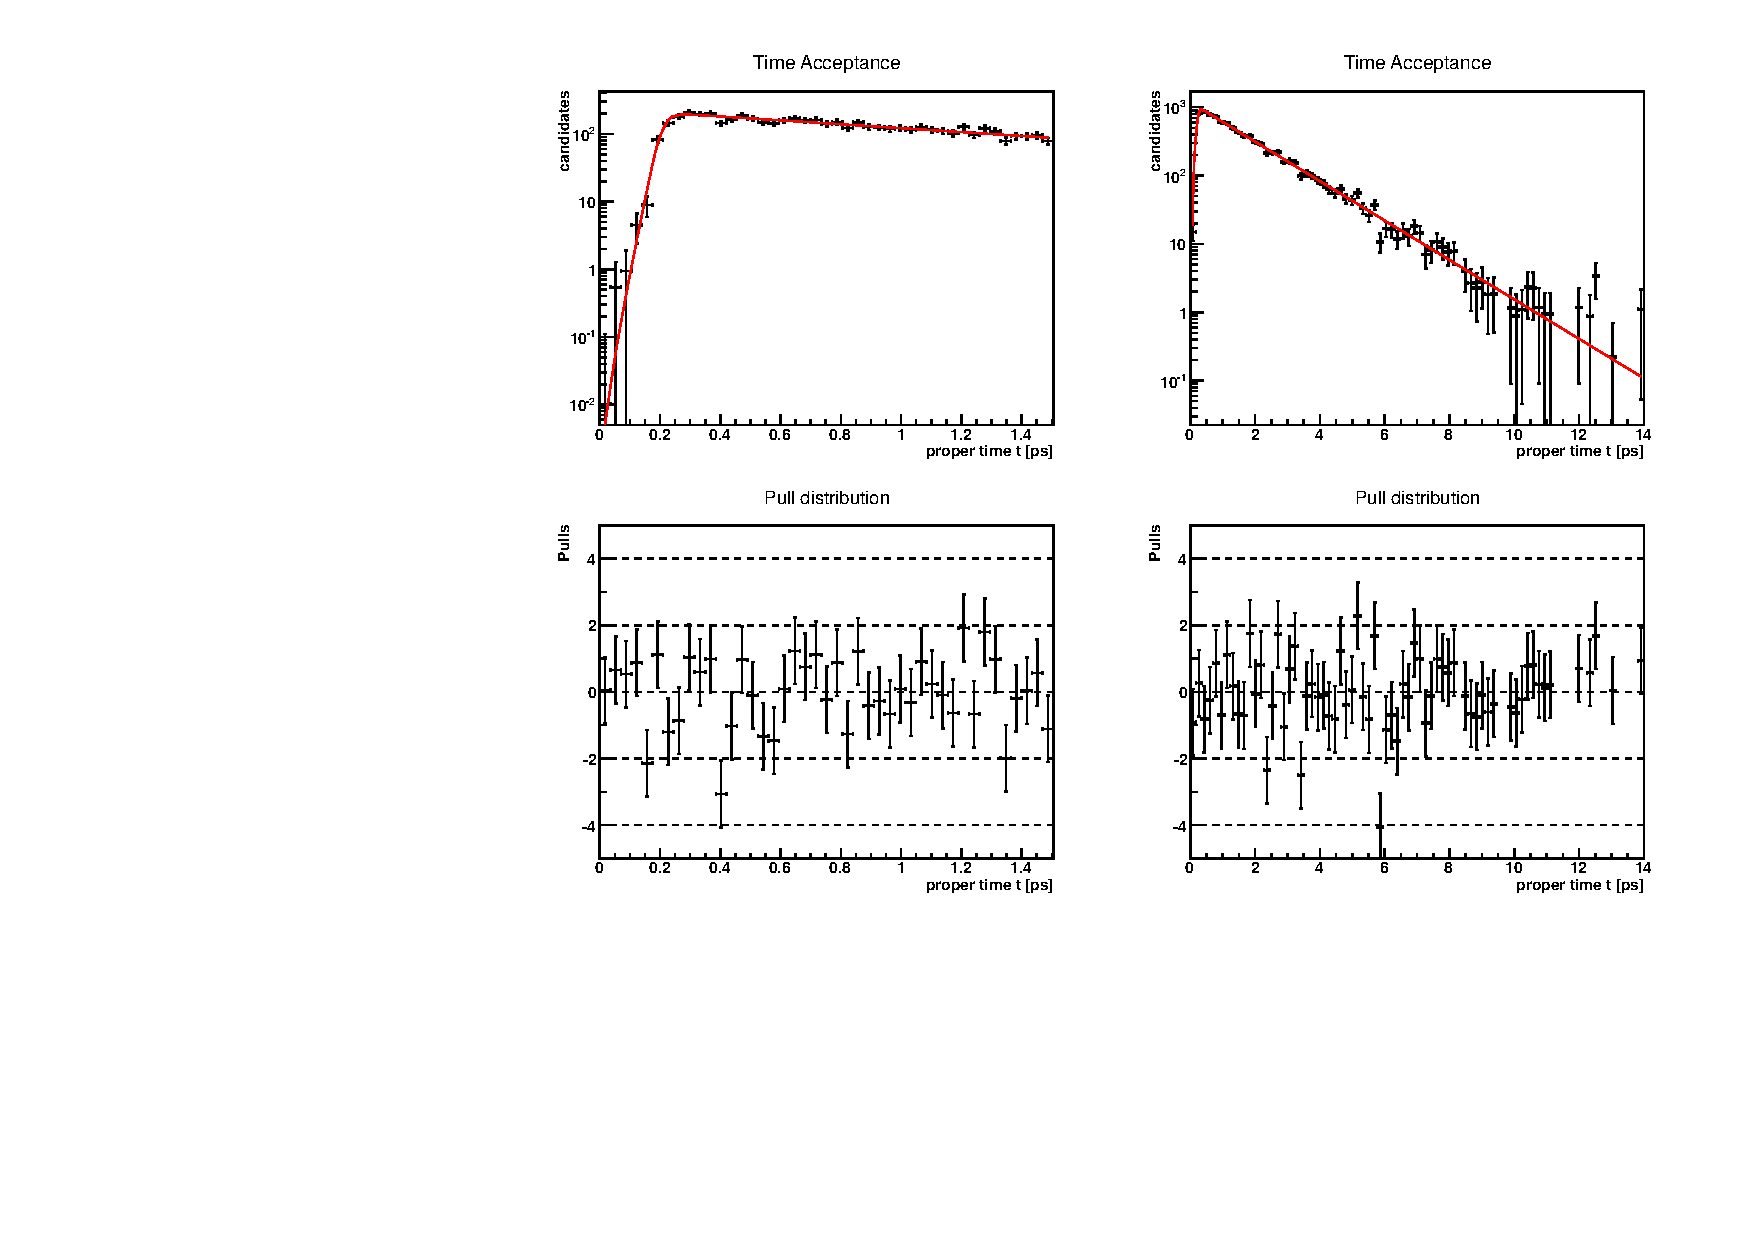
\includegraphics[width=\textwidth]{time_acceptance_fit}
\caption{Fit an die Flugzeit-Verteilung aller \Bd-Mesonen mit eingeschlossener Akzeptanzfunktion (oben) sowie die entsprechende Pull-Verteilung (unten). Links: kurzlebiger Zeitbereich ($t<1,5\pico\second$), Rechts: gesamtes Flugzeitspektrum ($0\ps < t < 14\ps$)}
\label{fig:fit_akzeptanz}
\end{figure}

\subsection{Bestimmung des Einflusses}
Durch den Cut auf die Lebensdauer bei $t = 0,3\ps$ in der Datenselektion spielt der Turn-On-Effekt im hier verwendeten Datensatz eigentlich keine Rolle. Dies wird dadurch deutlich, dass die Akzeptanzfunktion $\epsilon(0,3\ps) = 0,992$ und damit fast Eins ist. Auch am Ende des Analysebereichs beträgt die Akzeptanz noch $\epsilon(14\ps) = 0,905$. Daher liegt die Vermutung nahe, dass sich die Akzeptanz nicht gravierend auf das Fitergebnis auswirkt. Mit den in Kapitel \ref{kap:akzeptanz_bestimmung} bestimmten Parametern wird die zeitliche Akzeptanz bei der Erzeugung der Toys berücksichtigt, der anschließende Fit aber ohne Akzeptanzfunktion durchgeführt. Die zur Erzeugung verwendeten Parameter entsprechen ansonsten denen in Kapitel \ref{kap:fit_bias}.

\begin{figure}[hptb]
\centering
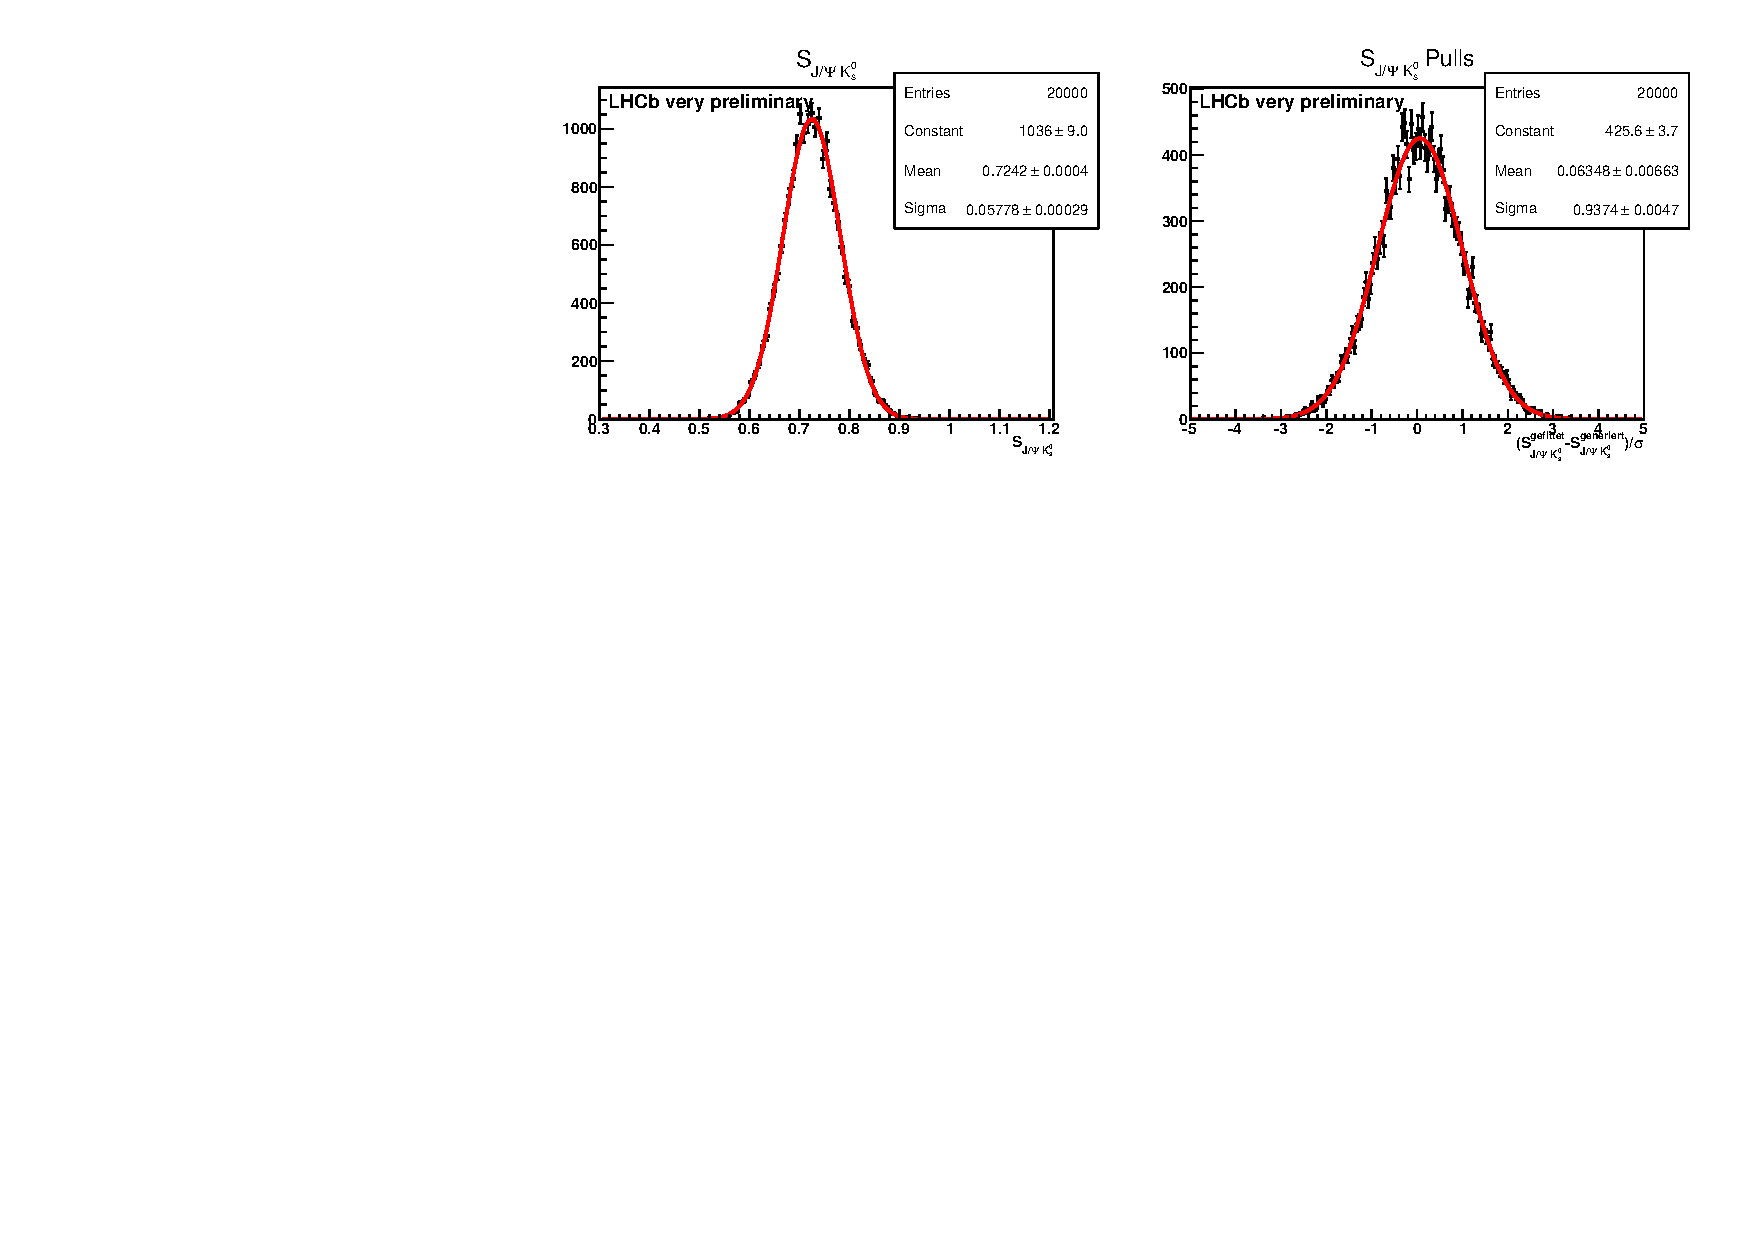
\includegraphics[width = \textwidth]{time_acceptance_toys}
\caption{Untersuchung des Einflusses einer zeitlichen Akzeptanz: Verteilung der aus der Toy MC Studie erhaltenen Amplituden $\SJPsi$ (links) sowie die dazugehörigen Pulls (rechts)}
\label{fig:toys_acceptance}
\end{figure}

Der Mittelwert der Pulls $\mu = 0,063 \pm 0,007$ (siehe Abb. \ref{fig:toys_acceptance}) ist kompatibel mit dem aus dem Fit Bias erhaltenen $\mu = 0,059 \pm 0,007$ und erzeugt dementsprechend keinen signifikanten zusätzlichen Bias. Damit ist die Vernachlässigung der zeitlichen Akzeptanz im Fit gerechtfertigt.



\section{Korrelation zwischen Masse und Eigenzeit}
Die sFit-Methode funktioniert dann gut, wenn der Untergrund der Massenverteilung eben ist und die Massenverteilung des Signals unabhängig von der gemessenen Eigenzeit ist. Es soll nun eine etwaige Korrelation zwischen Masse und Eigenzeit untersucht und der Einfluss auf $\SJPsi$ festgestellt werden. Dazu wird die Massenverteilung in vier verschiedenen Zeitbereichen gefittet, die Tabelle \ref{tab:mass_ct} zu entnehmen sind. Anschließend wird die gesamte Eigenzeitverteilung gefittet, dabei werden aber die Massenparameter des Signals auf die in den 4 Massenfits erhaltenen Werte fixiert. Die Ergebnisse des jeweiligen Fits sind ebenfalls in Tabelle \ref{tab:mass_ct} aufgeführt.

\begin{table}[hptb]
\centering
\caption{Einteilung der Eigenzeitbereiche sowie Fitresultate für $\SJPsi$ bei Fixierung der Masse auf die in den Zeitbereichen enthaltene Massenform. Weiterhin werden die Abweichung $\Delta\SJPsi$ vom regulären Datenfit und der Signalanzahl $N_{sig}$ eines jeden Eigenzeitbereichs genannt.}
\label{tab:mass_ct}
\begin{tabular}{c l r@{$\pm$}l c c}
\hline \hline
Nr. & Eigenzeitfenster des Massenfits & \multicolumn{2}{c}{$\SJPsi$} & $\Delta\SJPsi$ & $N_{sig}$\\ \hline
1 & $t \in [0.3, 0.7] \pico\second$ & 0,559 & 0,069 & -0,066 & 1898 \\
2 & $t \in [0.7, 1.5] \pico\second$ & 0,567 & 0,068 & 0,002 & 2773 \\
3 & $t \in [1.5, 3] \pico\second$ & 0,566 & 0,069 & 0,001 & 2710 \\
4 & $t \in [3, 14] \pico\second$ & 0,566 & 0,069 & 0,001 & 1490 \\ \hline \hline
\end{tabular}
\end{table}

Zur Abschätzung des Fehlers werden zunächst die Abweichungen $\Delta\SJPsi$ vom (noch verdeckten) Referenzwert aus dem regulären Eigenzeitfit $\SJPsi = 0,565 \pm 0,069$ berechnet und diese dann - gewichtet nach der Signalzahl $N_{sig}$ - quadratisch gemittelt:
\begin{align}
\delta\SJPsi^{m/t} = \sqrt{\frac{\sum N_i (\Delta\SJPsi)_i}{\sum N_i}} = 0,0031
\end{align}

\section{Eigenzeitauflösung}
Bei einer effektiven Eigenzeitauflösung von $\sigma_{eff} = (0,0665 \pm 0,0047)\ps$ im Vergleich zur \Bd-Oszillationsfrequenz $\delta m_d = (0,521 \pm 0.039)\hbar\ps$ erwartet man keine nennenswerten Effekte auf die Amplitude $\SJPsi$. Um überhaupt einen Effekt zu sehen, werden die Auflösungsparameter $\sigma_i$ um 20\% ihres Werte erhöht bzw. gesenkt und damit dann der Datensatz gefittet. Die größte Abweichung vom Referenzwert des regulären Eigenzeitfits wird als systematischer Fehler angenommen. Die Ergenisse finden sich in Tabelle \ref{tab:syst_resolution}.

\begin{table}[hptb]
\centering
\caption{Ergebnisse des Eigenzeitfits bei Variaton der Auflösungsparameter $\sigma_i$ um $\pm 20\%$.}
\label{tab:syst_resolution}
\begin{tabular}{l c c c r@{$\pm$}l c }
\hline \hline
Variation & $sigma_1$ & $sigma_2$ & $sigma_3$ & \multicolumn{2}{c}{$\SJPsi$} & $\Delta\SJPsi$ \\ \hline
$+20\%$ & 0,576 & 0,05275 & 0,1118 & xxx & xxx & xxx \\
$-20\%$ & 0,384 & 0,03517 & 0,0746 & xxx & xxx & xxx \\ \hline \hline
\end{tabular}
\end{table}

Es zeigt sich, dass eine exakte Bestimmung der Auflösung nicht von Nöten ist, da sie im Vergleich zu anderen Systematiken vor allem gegenüber der Flavour-Tagging Kalibration vernachlässigt werden kann. Dennoch wird ein sytematischer Fehler durch die Auflösung mit
\begin{align}
\delta\SJPsi^{res} = xxx
\end{align}
assoziiert.

\section{Gesamtsystematik}
Tabelle \ref{tab:syst_gesamt} fasst nochmals alle systematischen Unsicherheiten zusammen. Der Gesamtfehler wird durch quadratische Addition berechnet.

\begin{table}[hptb]
\centering
\caption{Zusammenfassung der systematischen Unsicherheiten}
\label{tab:syst_gesamt}
\begin{tabular}{l c }
\hline \hline
Effekt & $\delta\SJPsi$ \\ \hline
Fitmethode & xxx \\
Flavour-Tagging Kalibration & xxx \\
Eigenzeitakzeptanz & xxx \\
Korrelation Masse $\leftrightarrow$ Eigenzeit & xxx \\ 
Eigenzeitauflösung & xxx \\ \hline 
Gesamt & xxx \\ \hline \hline
\end{tabular}
\end{table}